\chapter{Temps de diffusion élastique}
\label{ch:TauS_PRL}

Dans les chapitres précédents, nous avons détaillé comment était produite notre onde de matière, et plus particulièrement l'utilisation de techniques de refroidissement à l'extrême nous permettant d'obtenir un condensat de Bose-Einstein assimilable à une onde plane $\etat{\mathbf{k}=0}$. Nous avons aussi discuté comment est généré notre désordre optique et nous nous sommes focalisés sur ses propriétés statistiques et spatiales.

À présent, nous allons nous concentrer sur la mesure du temps de diffusion élastique $\taus$, réalisée en 2015 lors de la thèse de Jérémie Richard \citep{richard2015propagation}. le temps de diffusion élastique a ainsi été étudié en fonction de l'amplitude du désordre $\VR$ et de l'énergie de l'onde (énergie cinétique, ou de manière équivalente son impulsion $k_{\mathrm{i}}$). Les résultats de cette étude ont donné lieu à une publication dans la revue \emph{Physical Review Letters} \citep{richard2019elastic}.


\section{Approximation de Born}
Dans cette section, nous allons nous concentrer sur la description du temps de diffusion élastique dans le régime de désordre faible. Ce régime perturbatif, appelé \emph{régime de Born}, fournit une image intuitive de la physique du désordre et reste le seul régime permettant d'obtenir des résultats quantitatifs.

\subsection{Temps de diffusion élastique dans le régime de désordre faible}
L'approximation de Born consiste à traiter l'effet du désordre $V(\mathbf{x})$ de manière perturbative\footnote{Une définition plus précise de l'approximation de Born basée sur le concept de \emph{Self-Energy} sera donnée dans le chapitre \ref{ch:TauS_NJP}.}.  Dans cette vision de désordre faible, on peut considérer la propagation dans le désordre comme une succession d'évènements de diffusion simple pour lesquels l'onde diffuse sur un diffuseur unique. L'étude du temps de diffusion élastique se concentre donc sur la dynamique d'un unique évènement de diffusion.



Dans le régime désordre faible, on peut considérer l'effet du désordre comme un couplage de l'état initial $\etat{\mathbf{k}_{\mathrm{i}}}$ à un continuum d'états d'impulsion $\etat{\mathbf{k}'}$ pour lesquels $\left| \mathbf{k}' \right| = \left| \mathbf{k}_{\mathrm{i}} \right| $ afin de satisfaire la conservation de l'énergie, les collisions étant élastiques. Cette situation est illustrée figure \ref{fig:illustration_contexte_taus}. 

\begin{figure}
\centering
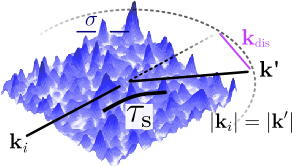
\includegraphics[scale=1]{Fig/TauS_PRL/illustration_contexte_taus.pdf}
\caption{\textbf{Illustration du temps de diffusion élastique dans l'approximation de Born.} L'onde plane initiale $\etat{\mathbf{k}_{\mathrm{i}}}$ expérience une collision dans le désordre et change d'impulsion $\etat{\mathbf{k}'}$. Les collisions avec le désordre étant élastiques, la conservation de l'énergie impose $\left|\mathbf{k}'\right|=\left|\mathbf{k}_{\mathrm{i}}\right|$. L'impulsion transférée $\mathbf{k}_{\mathrm{dis}}$ possède une borne supérieure en raison de la taille finie $\sigma$ des grains de speckle.}
\label{fig:illustration_contexte_taus}
\end{figure}


Dans cette image, l'évolution temporelle de l'état initial est donnée par une décroissance exponentielle 
\begin{equation}
n(\mathbf{k}_{\mathrm{i}},t)=n(\mathbf{k}_{\mathrm{i}},0) e^{-t/\taus} \text{ ,}
\end{equation}
où $t$ est le temps de propagation dans le désordre et le taux de décroissance $1/\taus$ est donné par la règle d'or de Fermi
\begin{equation}
\frac{\hb}{\taus^{\mathrm{Born}}}=2\pi \sum_{\mathbf{k}'}{\overline{\left |\left\langle \mathbf{k}' \left|  \hat{V} \right| \mathbf{k}_{\mathrm{i}} \right\rangle \right|^2} \delta(E_{\mathrm{k}'} - E_{\mathrm{k}_i})} \text{ ,}
\end{equation}
où $E_{\mathrm{k}}=\hb^2 k^2 /2m$ est l'énergie de l'onde plane $\etat{\mathbf{k}}$ de masse atomique $m$. L'interprétation de cette équation est aisée: la déplétion de l'état initial fait intervenir tous les états finaux permis par le potentiel qui respectent la conservation de l'énergie. 

Dans le cas d'un potentiel auto-moyennant, on peut montrer que le terme de couplage $\overline{|\langle \mathbf{k}'| \hat{V} | \mathbf{k}_{\mathrm{i}} \rangle|^2}$ est relié à la fonction de corrélation du potentiel de telle sorte que \citep{bernard2010transport}
\begin{equation}
\frac{\hb}{\taus^{\mathrm{Born}}}=2\pi \sum_{\mathbf{k}'}{\widetilde{C}(\mathbf{k}'-\mathbf{k}_{\mathrm{i}}) \delta(E_{\mathrm{k}'}  - E_{\mathrm{k}_i})} \text{ ,}
\label{eq:fermi_taus}
\end{equation}
où le spectre des fréquences spatiales du désordre $\widetilde{C}(\mathbf{k}_{\mathrm{dis}})$ est la transformée de Fourier de la fonction de corrélation du désordre $C(\Delta\mathbf{x})=\overline{V(\mathbf{x}) V(\mathbf{x}+\Delta\mathbf{x})}$ d'après le théorème de Wiener-Khintchine.

Le domaine de validité de l'approximation de Born peut être estimée d'une manière intuitive. En effet, le fait que l'état initial $\etat{\mathbf{k}_{\mathrm{i}}}$ possède un temps de vie $\taus^{\mathrm{Born}}$ fini se traduit par un élargissement de la distribution d'énergie de cet état dans le désordre de l'ordre de $\Delta E= \hb/\taus^{\mathrm{Born}}$. Pour valider l'approche perturbative, cette largeur doit être petite devant l'énergie initiale de l'onde $E_{\mathrm{k}_i}=\hb^2 k_{\mathrm{i}}^2 /2m$. On retrouve ainsi la condition de désordre faible $k_{\mathrm{i}}\ls^{\mathrm{Born}}\gg 1$ identifiable au critère de Ioffe-Regel. 

\subsection{Régimes de diffusion}
Comme nous l'avons montré dans le chapitre \ref{ch:Speckle}, le désordre illuminé sur les atomes est corrélé. En particulier, celui-ci possède une longueur de corrélation $\sigma$, définissant ainsi une fréquence spatiale caractéristique $\sigma^{-1}$ à la frontière entre des deux régimes de diffusion brièvement présentés dans la section \ref{sc:diffusion_classique}. 

En effet, la diffusion de l'état $\etat{\mathbf{k}_{\mathrm{i}}}$ vers un état $\etat{\mathbf{k}'}$ n'est possible que si la fréquence spatiale $\mathbf{k}_{\mathrm{dis}}=\mathbf{k}'-\mathbf{k}_{\mathrm{i}}$ est contenue dans le spectre du désordre. Pour des impulsions initiales faibles telles que $k_{\mathrm{i}}\ll\sigma^{-1}$, le désordre contient toutes les fréquences spatiales nécessaires pour diffuser l'onde dans toutes les directions (voir figure \ref{fig:desordre_2D}.a). Dans le cas contraire, où $k_{\mathrm{i}}\gg\sigma^{-1}$, les fréquences spatiales du désordre sont trop faibles pour satisfaire la condition de rétro-diffusion $\mathbf{k}_{\mathrm{dis}}=-2 \mathbf{k}_{\mathrm{i}}$. Dans ce cas de figure, l'essentiel de la diffusion se déroule aux alentours de la direction initiale de l'onde\footnote{Ce phénomène est analogue à la diffraction en optique. En effet, l'angle typique de diffraction d'un onde de nombre d'onde $k$ par un obstacle de taille $\sigma$ est donné par $\theta\sim 1/k\sigma$. Pour de grands nombres d'onde, la diffraction se fait dans un petit angle autour de la direction initiale de l'onde, tandis que pour de petits nombres d'onde la tâche de diffraction est étendue.}, on parle alors de régime de diffusion vers l'avant (voir figure \ref{fig:desordre_2D}.b). 

\begin{figure}
\centering
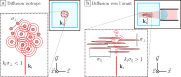
\includegraphics[width=\textwidth]{Fig/TauS_PRL/desordre_2D.pdf}
\caption{\textbf{Dynamique quasi-2D dans un speckle.} Les grains de speckle étant étendus selon la direction longitudinale, on peut trouver une configuration pour laquelle $k_{\mathrm{i}}\sigmal>1$, impliquant que la diffusion selon la direction $\vec{x}$ se fera essentiellement vers l'avant, et que $k_{\mathrm{i}}\sigmap<1$, impliquant une diffusion isotrope suivant les directions $\vec{y}$ et $\vec{z}$. De cette manière, on obtient une dynamique de diffusion quasi-2D, sans confiner le mouvement des atomes.}
\label{fig:desordre_2D}
\end{figure}

Plus précisément, nous avons vu au cours du chapitre \ref{ch:Speckle} que les grains de speckle ne sont pas isotropes et possèdent deux tailles caractéristiques $\sigmap$ suivant les directions transverses et $\sigmal$ selon la direction longitudinale. Il est donc possible de se placer dans une situation où la diffusion est isotrope dans le plan transverse ($k_{\mathrm{i}}\sigmap<1$) tandis que celle-ci se déroule majoritairement vers l'avant selon l'axe optique ($k_{\mathrm{i}}\sigmal>1$). Pour des temps de propagation dans le désordre de l'ordre de quelques collisions élastiques, la dynamique de la diffusion sera essentiellement bidimensionnelle\footnote{Avec nos paramètres expérimentaux usuels $k_{\mathrm{i}}\sim\SI{1}{\micro\metre^{-1}}$ et $\sigmal/2\sim\SI{2}{\micro\metre}$, il faut environ $N=(\pi k_{\mathrm{i}} \sigmal)^2 \sim 150$ collisions pour diffusion devienne isotrope \citep{denechaud2018vers}.}, sans devoir confiner le mouvement des atomes.


\subsection{Calcul du temps de diffusion élastique dans le régime de Born}

calculer $\taus$ en 2D et faire apparaître la fonction de Bessel modifiée. Juste montrer la comparaison au cas 3D pour montrer que le 2D est suffisant.


\section{Mesure du temps de diffusion élastique}
\subsection{Procédure expérimentale}
détailler comment ça se fait la manip.
Création d'un BEC, delta-kick pour obtenir $T\sim\SI{150}{\pico\kelvin}$.
Création du kick initial à l'aide d'un gradient magnétique, on obtient ainsi une onde plane $\etat{\mathbf{k}_{\mathrm{i}}}$.
On quench le désordre, avec un désaccord d'au moins 1 TeraHertz, qui donne un potentiel conservatif qui conserve les mêmes propriétés selon qu'il soit désaccordé vers le rouge ou vers le bleu.
Ensuite on fait un grand temps de vol pour obtenir la distribution d'impulsion. jusqu'à 300ms.
Imagerie par fluo.

\subsection{Extraction du temps de diffusion élastique}
Observation de la déplétion du pic initial (pas de propagation dans le désordre) au cours de la propagation dans le désordre. Formation d'un cercle témoignant du caractère élastique des collisions (conservation de l'énergie). Taus= temps de déplétion de l'état initial vers les autres états de l'anneau avec une décroissance exponentielle. On a tout extrait par un ajustement exponentiel, même si on sait que c'est pas valide partout. On a fait ça parce que on a pas observé de déviation expérimentale à ce comportement.
Même procédure pour les traitements numériques. ajustement exponentiel local sur les mêmes plages de données que pour les expérimentales.
Montrer les résultats.
\subsection{Calibration de l'amplitude du désordre}
Excellent accord entre les données expérimentales et les données numériques. Du coup, on se sert de cet accord pour calibrer l'amplitude du désordre expérimental. Plus particulièrement, on utilise les données pour $k_{\mathrm{i}}=0.74 \sigma^{-1}$ pour apporter une correction à $\VR {}_{\mathrm{,expérimental}}$: $\alpha=1.29\pm0.02$.


\section{Comportement du temps de diffusion élastique}
\subsection{Régime de Born}
\subsection{Déviations au régime de Born}
\subsection{Départ quadratique}